\documentclass{article}
\usepackage{amsmath}
\usepackage{listings}
\usepackage[utf8]{inputenc}
\usepackage{graphicx}
\usepackage{url}
\usepackage{placeins}

\graphicspath{ {../results/} }

\lstset{
	basicstyle=\footnotesize,
	numbers=left,
	tabsize=3,
	title=\lstname,
	breaklines=true
}

\addtolength{\oddsidemargin}{-.875in}
\addtolength{\evensidemargin}{-.875in}
\addtolength{\textwidth}{1.75in}

\addtolength{\topmargin}{-.875in}
\addtolength{\textheight}{1.75in}

\title{Lernverfahren autonomer Roboter - Übung 6}
\author{Tobias Hahn\\ 3073375}	
	
\begin{document}
\maketitle
\newpage
\section*{Übung 6}
\section{Hierarchical Clustering}

\section{Gradient Descent}
Hier gibt es nicht viel zu erklären: Für die Anzahl der Iterationen wird der Parametervektor um den Gradienten mit der gewünschten Lernrate angepasst, wobei die jeweiligen Gewichtsvektoren auch noch in einer Liste gespeichert werden wenn ein Pfad gewünscht ist.

\section{Gradient Descent for Linear Regression}
\subsection{Results}
\begin{lstlisting}[title=Konsolenoutput]
alpha = 0.0001:	 w* = array([ 0.41939905,  0.68353485]), SSE(w*) = 53.2682
alpha = 0.001:	 w* = array([ 0.69059681,  0.6936927 ]), SSE(w*) = 49.6219
alpha = 0.002:	 w* = array([ 0.69061859,  0.6936935 ]), SSE(w*) = 49.6219
alpha = 0.0025:	 w* = array([   538.35090254, -14615.23032604]), SSE(w*) = 8.97992e+10
\end{lstlisting}

\begin{figure}[h]
    \centering
    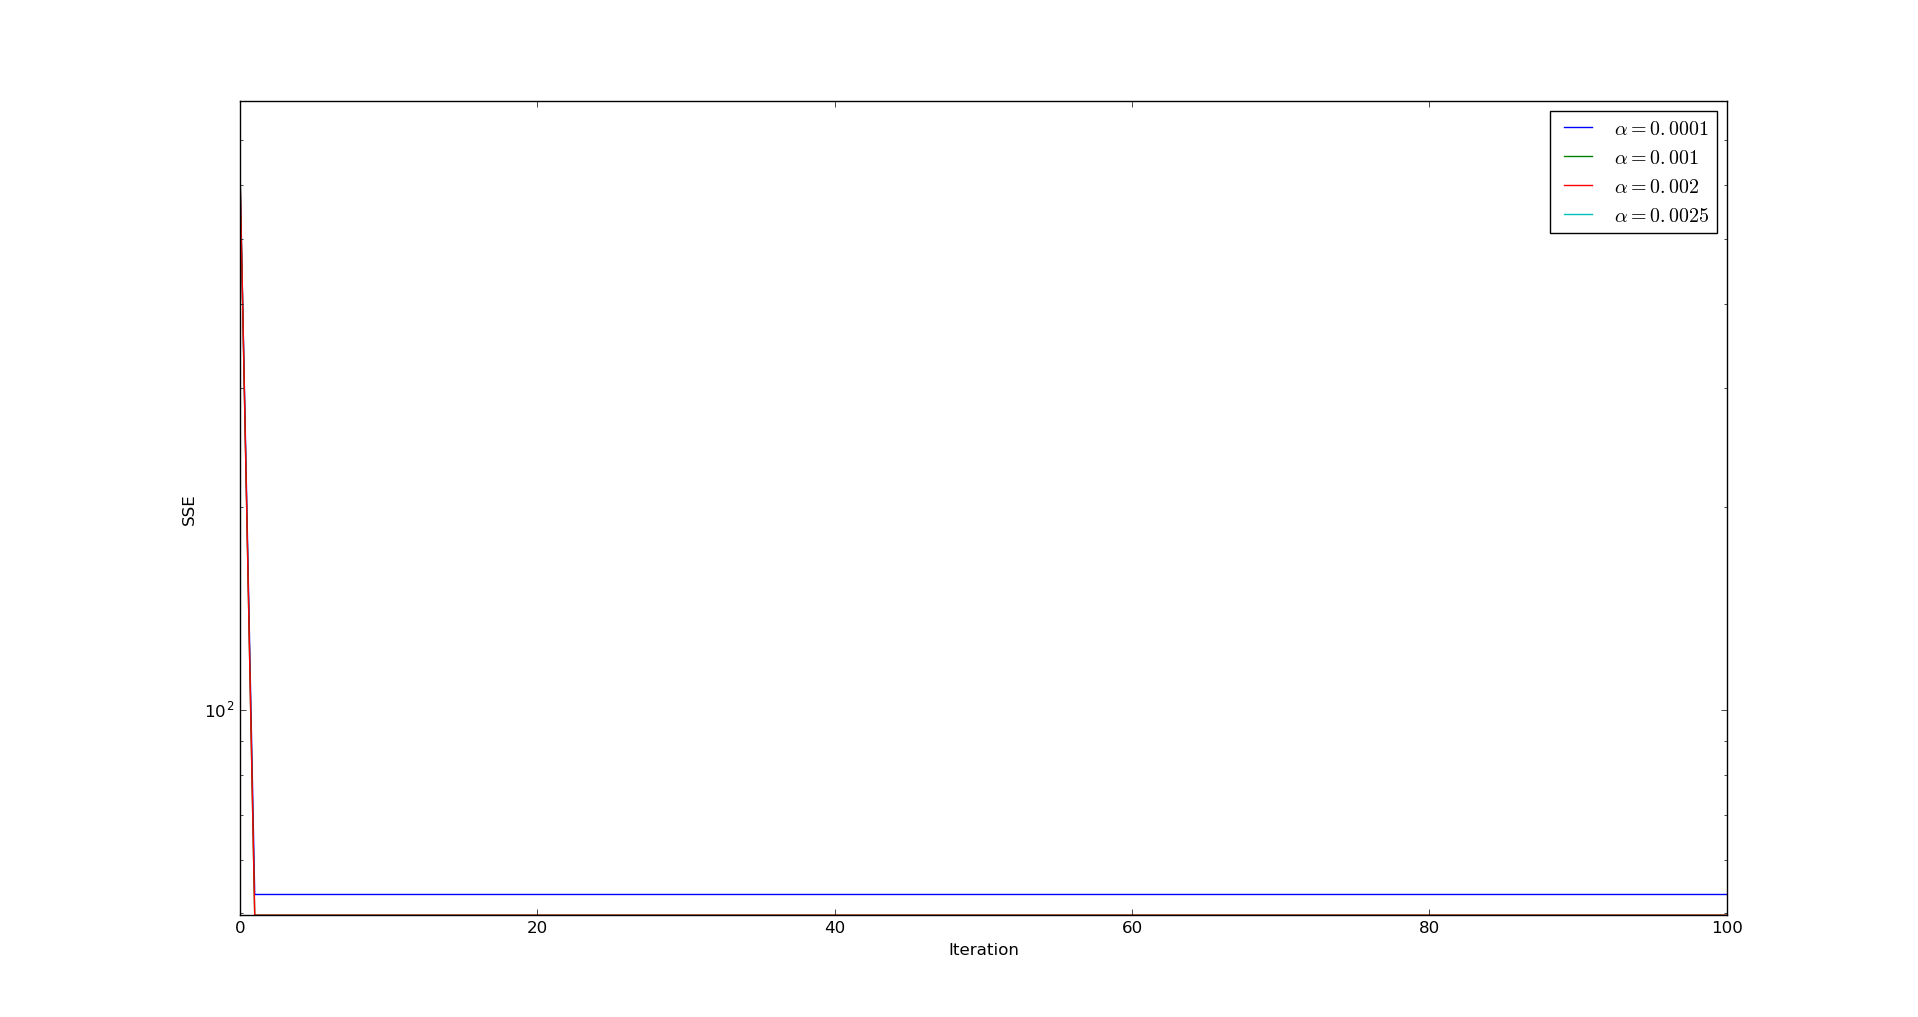
\includegraphics[width=\textwidth]{linear_regression.png}
    \caption{Die Sum of Squared Errors für alle Parametervektoren im Lösungspfad}
    \label{fig:sse}
\end{figure}
\FloatBarrier

\subsection{Diskussion}
Bei der Lernrate gibt es zwei Gefahren: Wird sie zu klein gewählt, dauert es sehr lange bis der Algorithmus zu einem Ergebnis kommt. Wird sie zu groß gewählt kann es vorkommen dass der Algorithmus hin und her springt, also den Fehler u.U. dauernd vergrößert. Das kommt daher dass der Parametervektor das Minimum, in dessen Richtung der Gradient zeigt so weit überspringt dass der Fehler wieder größer wird. Dieser Effekt verstärkt sich bei Linearer Regression von selbst, da der Gradient bei größerem Fehler größer ist, also man beim nächsten Schritt noch größer wird und so weiter.

Bei unserem Beispiel sehen wir den ersten Effekt bei einer Lernrate von 0.0001 - die Fehlerrate ist noch relativ groß, da 100 Iterationen bei so einer geringen Fehlerrate zu wenig sind. Der zweite Effekt zeigt sich bei der Lernrate von 0.0025 - die Lernrate ist zu groß, der Parametervektor springt über das Ziel hinaus und schaukelt sich so in immer höhere Fehlerbereiche hoch.

Die zwei Lernraten in der Mitte sind gut gewählt und erreichen das Minimum. Hier wäre jedoch 0.002 vorzuziehen, da es schneller konvergiert - bei fixer Epochenanzahl nicht wirklich ein Kriterium, wenn man den Algorithmus jedoch bei Konvergenz stoppen lässt schon.
\end{document}
